\section{Fractures and sorption}

File: \texttt{05\_frac\_sorption.yaml}

\subsection{Description}

This is a variant of \texttt{04\_frac\_diffusion.yaml}. Instead of
diffusion we consider advective transport with equilibrial sorption.

\subsection{Input}

Flow123d provides several types of sorption (linear, Langmuir and
Freundlich isotherm). Each substance can be assigned its own sorption
type. In this test, the transport of three substances is computed:
Iodium without sorption, Radium with liner sorption and Selenium with
Langmuir isotherm. The solvent density and solubility was set to 1.
Initial condition of solid was set to zero; rock density to 1 and
parameter of liner and Langmuir isotherm was set to 0.6.

\begin{verbatim}
reaction_term: !Sorption
  substances:
    - I
    - Ra-lin
    - Se-lang
  solvent_density: 1.0
  solubility: [ 1.0, 1.0, 1.0 ]
  input_fields:
    - region: ALL
      init_conc_solid: 0
      rock_density: 1.0
      sorption_type:
        - none           
        - linear           
        - langmuir
      isotherm_mult: 0.6          
      isotherm_other: 0.4
\end{verbatim}

In fact, the fields \texttt{init\_conc\_solid}, \texttt{isotherm\_mult},
\texttt{isotherm\_other} can have different values for each substance.
In that case we define them as YAML arrays.

\subsection{Results}

Figure \ref{fig:sorp_res} depicts the influence of linear and Langmuir
isotherm on the transport of substances. The substance I without
sorption flows out of the fracture fastest and the substance Ra flows
out slowest.

\begin{figure}[htbp]
\centering
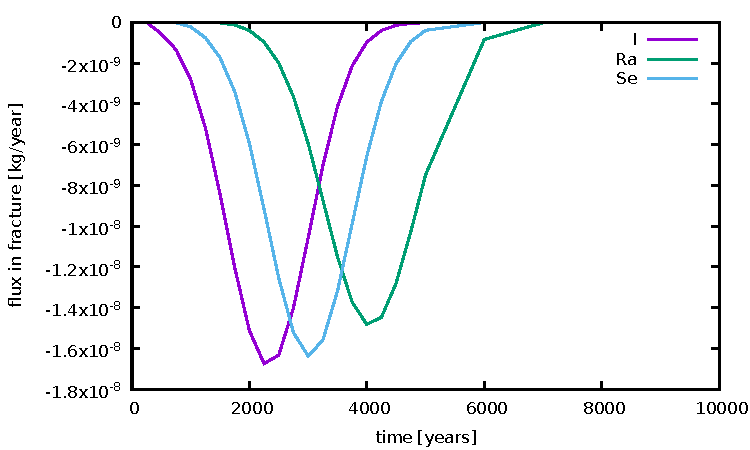
\includegraphics{tutor_figures/05_mass_flux.pdf}
\caption{Results of sorption.\label{fig:sorp_res}}
\end{figure}
